\section{Testy wydajnościowe}

\subsection{Test 1}

\subsubsection{Test a}

Kolejnym przypadkiem jest zbadanie rzadkich wielomianów, nieposiadających pierwiastków całkowitych. By zapewnić ten ostatni element, najłatwiejszym sposobem jest konstrukcja wielomianu postaci $ax^{2k}+b$, gdzie $a \in R_+, b \in R, k \in Z_+$. Dzięki temu, mamy pewność, że wielomian nie posiada pierwiastków całkowitych, a dodatkowo ma najmniejszą możliwą liczbę niezerowych współczynników.

Teoretycznie, wielomiany rzadkie powinny się charakteryzować największą dysproporcją w wydajności pomiędzy typami PolynomialMap i PolynomialVector, na korzyść tego pierwszego. Jest to spowodowane faktem, że to właśnie w tym przypadku, odsetek zerowych współczynników jest największy. Czynnik ten powinien bardzo negatywnie wpływać na czas znajdowania pierwiastków, a w tym przypadku na stwierdzenie, o ich braku. Zapoznajmy się z wynikami testów, by zweryfikować postawioną powyżej tezę.

\begin{table}
	\caption{Porównanie czasów obu typów wielomianów dla rzadkich wielomianów parzystego stopnia}
	\begin{tabular}{ |p{3.5cm}|p{3cm}|p{3cm}|p{3.5cm}|} 
		\hline
		Testowany wielomian & Czas dla PolynomialMap [s] & Czas dla PolynomialVector [s] & Współczynnik czasów \\
		\hline
		$W(x) = x^{100} + 1$ & 0.049 & 2.278 & 46.49 \\
		$W(x) = x^{200} + 1$ & 0.102 & 9.438 & 92.53 \\
		$W(x) = x^{400} + 1$ & 0.221 & 40.432 & 182.95 \\
		$W(x) = x^{800} + 1$ & 0.525 & 184.608 & 351.63 \\
		$W(x) = x^{1600} + 1$ & 1.374 & 912.716 & 664.28 \\
		$W(x) = x^{3200} + 1$ & 4.153 & 5125.106 & 1234.07 \\
		\hline
	\end{tabular}
\end{table}

\subsubsection{Test b}

Teraz rozpatrzmy sytuację, w której ponownie mamy do czynienia z wielomianem rzadkim, o którym wiemy, że posiada przynajmniej jeden pierwiastkek rzeczywisty. By to zapewnić, wystarczy skonstruować wielomian w postaci $ax^{2k+1}+b$, gdzie $a \in R\setminus\{0\}, b \in R, k \in Z_+$. Jak wiemy, na podstawie przedstawionego w drugim rozdziale twierdzenia, każdy wielomian stopnia nieparzystego posiada przynajmniej jeden pierwiastek rzeczywisty. 

Wydaje się, że podobnie jak w przypadku wielomianów nieposiadających pierwiastków, również w tym, czas znajdowania pierwiastków dla typu PolynomialMap powinien być znacznie krótszy niż dla PolynomialVector. Natomiast, czy aby na pewno, tak jest? Rozważmy poniższy przykład.
Postarajmy się zbudować ciąg Sturma dla wielomianu $x^{101}+1$. Zacznijmy od obliczenia pochodnej.
$(x^{101}+1)'=101x^{100}$
Obliczona wartość jest drugim elementem ciągu Sturma. Obliczmy resztę z dzielenia dwóch pierwszych wielomianów tego ciągu: \\
\begin{equation*}
\begin{split}
&\frac{1}{101}x \\
\hline
&(x^{101}+1) : (x^{100}) \\
&-x^{101} \\
\hline
&1
\end{split}
\end{equation*}
Trzecim i jednocześnie ostatnim wyrazem ciągu Sturma jest więc $-1$, czyli wartość przeciwna do otrzymanej reszty. Dysponujemy zatem trzy elementowym ciągiem Sturma o elementach ${x^{101}+1, 101x^{100}, -1}$. Obliczmy teraz liczbę zmian znaków dla $-\infty$ i $+\infty$. W prawym krańcu przedziału będą to wartości $+,+,-,$ zaś w lewym $-,+,-.$ Otrzymaliśmy jedną zmianę znaku dla $-\infty$ i dwie zmiany dla $+\infty$. Oznacza to, że liczba pierwiastków rzeczywistych jest równa różnicy tych zmian w lewym i prawym krańcu, czyli w tym przypadku wynosi $1$.

Jak widać, dwa z trzech elementów ciągu Sturma to rzadkie wielomiany wysokich stopni. Na takiej podstawie, wydaje się, że powyższa teza została potwierdzona. Jednocześnie jednak, warto zauważyć, że dla tego rodzaju wielomianów liczba koniecznych operacji jest niewielka, z uwagi na znikomą liczbę elementów ciągu Sturma. Wydaje się zatem, że to właśnie ich liczba bezpośrednio wpływa na czas znajdowania pierwiastków, a ich charakterystyka, czyli liczba niezerowych współczynników ma największe znaczenie dla wydajności obu typów wielomianów. Sprawdźmy, czy wyniki testów potwierdzają powyższą teorię.

\begin{table}
	\begin{tabular}{ |p{3.5cm}|p{3cm}|p{3cm}|p{3.5cm}|} 
		\hline
		Testowany wielomian & Czas dla PolynomialMap [s] & Czas dla PolynomialVector [s] & Współczynnik czasów \\
		\hline
		$W(x) = x^{101} + 1$ & 0.049 & 2.278 & 46.49 \\
		$W(x) = x^{201} + 1$ & 0.102 & 9.438 & 92.53 \\
		$W(x) = x^{401} + 1$ & 0.221 & 40.432 & 182.95 \\
		$W(x) = x^{801} + 1$ & 0.525 & 184.608 & 351.63 \\
		$W(x) = x^{1601} + 1$ & 1.374 & 912.716 & 664.28 \\
		$W(x) = x^{3201} + 1$ & 4.153 & 5125.106 & 1234.07 \\
		\hline
	\end{tabular}
\end{table}

\begin{figure}[h]
	\caption{Czasy działania dla rzadkich wielomianów nieparzystego stopnia dla PolynomialMap}
	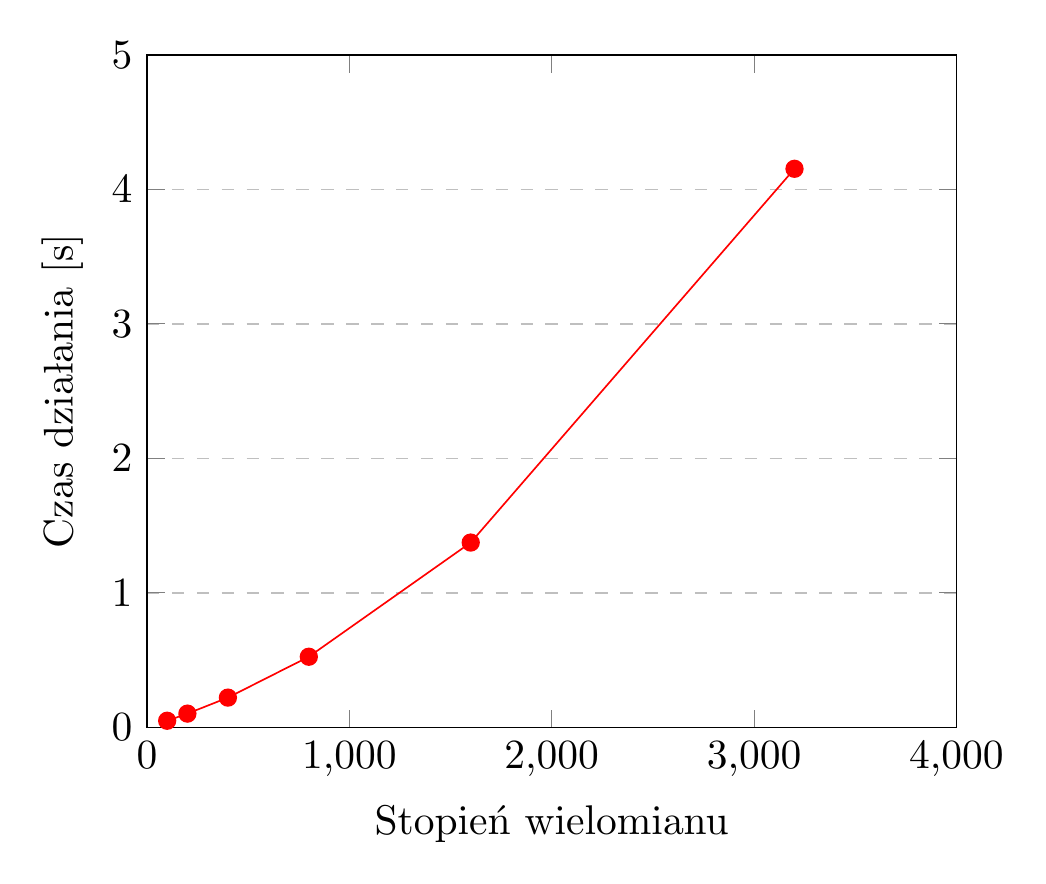
\begin{tikzpicture}[scale=1.5]
	\begin{axis}[
	xlabel={Stopień wielomianu},
	ylabel={Czas działania [s]},
	xmin=0,xmax=4000,
	ymin=0,ymax=5,
	ymajorgrids=true,grid style=dashed
	]
	
	\addplot[color=red,mark=*]
	coordinates {
		(100, 0.049)
		(200, 0.102)
		(400, 0.221)
		(800, 0.525)
		(1600, 1.374)
		(3200, 4.153)
	};
	\end{axis}
	\end{tikzpicture}
	\caption{Porównanie czasów obu typów wielomianów dla rzadkich wielomianów nieparzystego stopnia}
\end{figure}

\subsection{Test 3}

Na początku zastanówmy się, jak sprawić, by liczba elementów ciągu Sturma była jak największa. Pozwoli to nam, na zmaksymalizowanie liczby operacji na wielomianach danego stopnia. Aby to zrobić, najłatwiej jest zapewnić, by wielomian miał liczbę pierwiastków rzeczywistych równą lub zbliżoną w stosunku do jego stopnia. Jak wiemy, liczba ta jest równa różnicy liczby zmian ciągu Sturma w obu przedziałach, a jej wartość jest ograniczona przez liczbę wyrazów tego ciagu. Wynika z tego, że liczba elementów ciagu Sturma jest zawsze większa od liczby pierwiastków.

Teraz zastanówmy się, jak skonstruować wielomian, który zawiera liczbę różnych pierwiastków równą jego stopniowi. Intuicyjne utworzenie wielomianu, podając jego kolejne współczynniki jest niemożliwe dla wysokich stopni.

Rozwiązaniem jest więc przedstawienie go w postaci czynników, wskazując jego kolejne pierwiastki. Przykładowo wielomian W, o stopniu $k$, możemy przypisać pierwiastki, będące kolejnymi dodatnimi liczbami całkowitymi, ustalając jego wartość jako $W(x)=(x-1)*(x-2)*(x-3)*...*(x-(k-2))*(x-(k-1))*(x-k)$, gdzie $k$ jest stopniem wielomianu.

Przetestujemy więc wielomiany powyższej postaci. Z powodu ograniczeń czasowych zdecydowałem się w tym teście na badanie wielomianów niższych stopni, niż w pozostałych przypadkach. Zapoznajmy się z rezultatami opisanego eksperymentu.

TODO
